\documentclass[dvipdfmx]{article}
\usepackage[dvipdfmx]{graphicx}
\usepackage{amsmath, amssymb}
\usepackage{mathtools}
\usepackage{here}
\begin{document}
\title{Weekly Report}
\author{Riku Gondow}
\maketitle
\section{Progress}
\begin{itemize}
    \item Check the accuracy of Triple Joint Loss\cite{TJL}
    \item Read "Proportional Similarity-Based Openmax Classifier for Open Set Recognition in SAR Images"\cite{PS}
\end{itemize}
\section{Result}
\subsection{Softmax + Center Loss}
The equations for Softmax Loss and Center Loss are shown below. Softmax Loss increases the inter-class variance, while Center Loss enhances the intra-class aggregation. The sum of Losses uses the hyperparameter $\alpha$ to balance the two Losses.
\begin{equation*}{L_{{\text{Softmax }}}} = \frac{1}{N}\sum\limits_{i = 1}^N 1 - \log \frac{{{e^{\left\| {{{\mathbf{w}}_{yi}}} \right\|*\left\| {{{\mathbf{x}}_i}} \right\|*\cos {\theta _{yi}} + {{\mathbf{b}}_{yi}}}}}}{{\sum\limits_{j = 1}^C {{e^{\left\| {{{\mathbf{w}}_j}} \right\|*\left\| {{{\mathbf{x}}_i}} \right\|*\cos {\theta _j} + {{\mathbf{b}}_j}}}} }}\tag{1}\end{equation*}

\begin{equation*}{L_{{\text{Center }}}} = \frac{1}{2}\sum\limits_{i = 1}^N {{{\left\| {{\mathbf{x}}_i^j - {{\mathbf{c}}^j}} \right\|}_2}} ,(j = 1,2, \ldots ,C)\tag{2}\end{equation*}

\begin{equation*}{L_{{\text{Total }}}} = {L_{{\text{Softmax }}}} + \alpha {L_{{\text{Center }}}}\end{equation*}

In formula (1), $C$ is the total number of categories in the training set. $w_j, w_{yi}, b_j, b_{yi}$ is the weight matrixes and bias terms of the last fully connected layer of the network, $\theta_j$ is the angle between the weight vector and the feature vector in the high dimensional space.

In formula (2), $N$ is the number of samples of the $j$th class, $x_i^j$ represents the $i$th sample belonging to the $j$th class and $c^j$ represents the class center of the $j$th class.


\begin{figure}[H]
\begin{center}
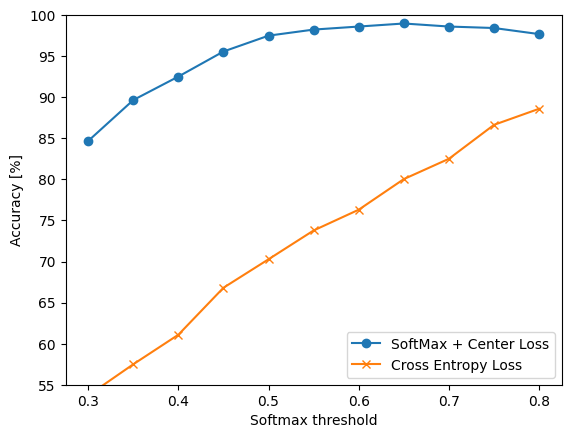
\includegraphics[width=\linewidth]{./img/soft_center.png}
\end{center}
\caption{Comparison of using Cross Entropy and Softmax + Center for loss function}
\end{figure}

Here is a figure. The figure1 shows a comparison of using Cross Entropy and Softmax + Center for loss function.
From Figure 1, we can see that higher accuracy is achieved for all threshold values when Softmax+Center is used than when Cross Entropy is used.

\begin{table}[H]
\caption{Comparison with two baselines}
\centering
\begin{tabular}{cccc}
\hline
Condition & Method & Known/Unknown & Accuracy \\
\hline
Open set & Yan et al.\cite{ddlm} (DDLM) & 15/15 & 93.57\% \\
& Xing et al.\cite{xing} & 15/15 & 94.35\% \\
& \textbf{Softmax + Center Loss} & 15/15 & 98.98\% \\
\hline
\end{tabular}
\end{table}

The table1 above shows the comparison between the two baselines. The table shows that the proposed method with Softmax and Center Loss outperforms the two methods.

\subsection{Triple Joint Loss(Softmax + Center + Large Margin Cosine Loss)}
The equations for Cosine Loss and Triple Joint Loss are shown below. Cosine loss enhances the intra-class aggregation and the inter-class dispersion. 

\begin{equation*}{L_{{\text{Cosine }}}} = - \frac{1}{N}\sum\limits_{i = 1}^N {\log } \frac{{{e^{s\left( {\cos {\theta _{yi}} - m} \right) + {{\mathbf{b}}_{yi}}}}}}{{{e^{s\left( {\cos {\theta _{yi}} - m} \right) + {{\mathbf{b}}_{yi}}}} + \sum\limits_{j = 1,j \ne {y_i}}^C {{e^{s\cos {\theta _j} + {{\mathbf{b}}_j}}}} }}\tag{3}\end{equation*}

\begin{equation*}{L_{{\text{Triple Joint }}}} = {L_{{\text{Softmax }}}} + \alpha {L_{{\text{Center }}}} + {L_{{\text{Cosine}}}}\end{equation*}

We set $||w_{yi}|| = 1, ||x_i|| = s$ in formula (1). It can be seen that after the introduction of s, the classification result is only affected by $\theta_{yi}$, the angle between the weight vector and the feature vector. $m$ is the cosine margin parameter that needs to be optimized
according to the training samples. The introduction of $m$ modifies the decision boundary of the neural network.
Finally, we combine the Softmax loss, the Center loss, and the Cosine loss to form Triple Joint Loss.

\begin{figure}[H]
\begin{center}
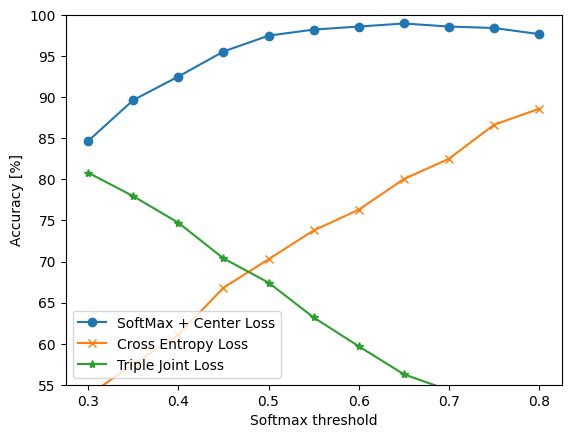
\includegraphics[width=0.9\linewidth]{./img/triple_joint.png}
\end{center}
\caption{Comparison of using three different losses for loss function}
\end{figure}

Here is a figure. The figure2 shows a comparison of using three different losses for loss function.
From the figure, we can see that Triple Joint Loss is less accurate than Softmax + Center Loss for all threshold values.

\subsection{Discussion}
For noisy datasets, the method combining Triple Joint Loss and Openmax-based method may have high robustness. This is because the 98.98\% accuracy was achieved on a low-noisy dataset, where the known labels can be classified fairly accurately and the Softmax functions output for the known labels is almost 1.

Also, Triple Joint Loss still has room to improve its accuracy by adjusting hyperparameters such as $\alpha, s,$ and $m$.

\section{Openmax vs Proportional Similarity Openmax}
In this section, we explain the differences between Openmax and PS Openmax based on the paper[2]. OpenMax is executed in the flow of Algorithm 1 -> 2 (model calibration -> OpenMax score calculation).
First, the model calibration is as follows:
\begin{figure}[H]
\begin{center}
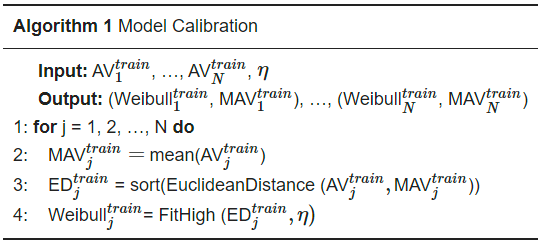
\includegraphics[width=0.8\linewidth]{./img/openmax1_algo.png}
\end{center}
\end{figure}

In the SoftMax layer, the output vector of the last layer of fully connected layers is typically used. This vector is called the \textbf{Activation Vector}. $AV_1^{train}$ (Activation Vector) represents the activation vector of the image (input) of the first class out of N classes. $\eta$ is a hyperparameter that determines how many of the distance values are included in the OpenMax score calculation. The line2 computes the average activation vector for each Known N classes.
This is performed using the FitHigg function and Weibull distribution of LibMR, which is a publicly available library, for maximum likelihood estimation.
Finally, Algorithm 1 returns the Weibull model and the MAV computed on N Known classes.

Next, the algorithm2 is as follows:
\begin{figure}[H]
\begin{center}
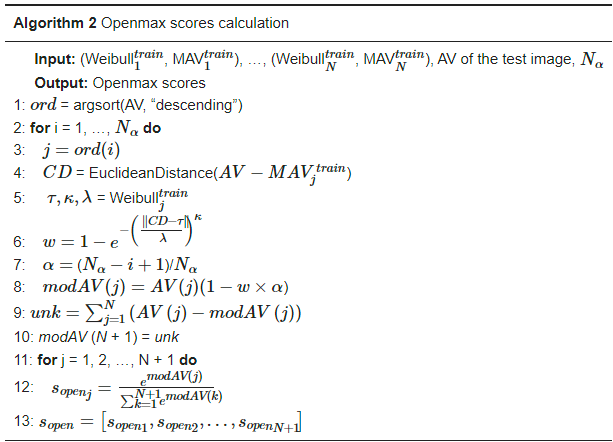
\includegraphics[width=\linewidth]{./img/openmax2_algo.png}
\end{center}
\end{figure}
From lines 1 to 9, The Openmax subtracts a portion from each element of AV based on the similarity of the test image and the respective training class, sums the subtracted values, and forms a modified AV with one more element appended to its end to represent the unknown class.
The N+1th class is then added as unknown at line 10, and the rest of the calculation is the same as SoftMax for the N+1 classes.

\newpage
Then, the Proportional Similarity-based Openmax is as follows:
\begin{figure}[H]
\begin{center}
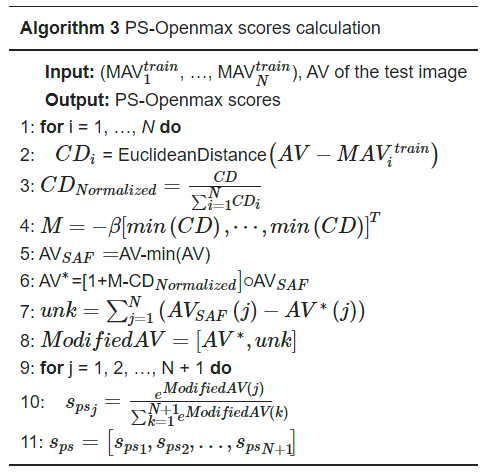
\includegraphics[width=0.8\linewidth]{./img/openmax3_algo.png}
\end{center}
\end{figure}

In algorithm3, the MAV (Mean Activation Vector) is computed in the same way as in OpenMax, forming the Euclidean channel distance vector $(CD)$ from all classes in lines 1 and 2.
In line 3, the normalized channel distance vector $(CD_{normalized})$ is computed, effectively avoiding the situation where the absolute value of the last element of the AV becomes too large; in OpenMax1, no interrelationship between the channel distance values is considered, and the channel distance values are used independently to modify the corresponding elements of AV.
In line 4, $min(CD)$ is repeated to form an $N \times 1$ vector, and $\beta \in (0,1)$ as a hyperparameter is used to balance between the minimum channel distance and the two elements of the normalized channel distance vector.
In line 5, a vector-type activation function $AV_{SAF}$ (supplementary activation function) is computed to ensure that each element of AV is not negative.

The proposed method modifies $AV_{SAF}$ on an element-by-element basis using two elements. They are the minimum channel distance M and the normalized channel distance vector $CD_{normalized}$ using the hadamard product $(\circ)$; (see line 6 of Algorithm 3).
By computing the sum of the subtraction between $AV_{SAF}$ and $AV*$ , a new element is formed (see line 7 of Algorithm 3). Like the original Openmax, the new element is added to the end of the modified AV (see line 8 of Algorithm 3), and the modified AV is mapped to the probability region to produce the PS-Openmax score (see lines 9-11 of Algorithm 3).

The PS (proportional similarity)-Openmax approach substitutes the tail fitting procedure with a proportional similarity measure and uses the relationship between the channel distance values to prevent new elements from always having too large negative or too large positive values There is also no need to adjust hyperparameters such as $\eta$ or $N_{\alpha}$.


With 10-images open set (called MSTAR dataset, known:8, unknown:2), openmax achieves 90\% accuracy and PS-Openmax 93\% accuracy. 

\section{Next Plan}
\begin{itemize}
    \item Visualize the feature mapping of output when using Softmax and Center Loss to see the effect of the loss
    \item Implement Openmax and Proportional Similarity-based Openmax
    \item Check the noisy data acquired in our lab
\end{itemize}
\begin{thebibliography}{99}

\bibitem{TJL} Y. Yang, B. Huang and Z. Ni, "Open-set Person Identification with Triple-Joint Loss Based on Radar Gait Micro-Doppler Signatures," 2022 7th International Conference on Intelligent Computing and Signal Processing (ICSP), 2022, pp. 1787-1791.
\bibitem{PS} Giusti E, Ghio S, Oveis AH, Martorella M. Proportional Similarity-Based Openmax Classifier for Open Set Recognition in SAR Images. Remote Sensing. 2022; 14(18):4665.
\bibitem{ddlm} Yan, Baiju, et al. ”Heart signatures: Open-set person identification based on cardiac radar signals.” Biomedical Signal Processing and Control 72 (2022): 103306.
\bibitem{xing} Zelin Xing, Mondher Bouazizi and Tomoaki Ohtsuki. Deep Learning-based Open-set Person Identification using Radar Extracted Cardiac Signals. 
\end{thebibliography}
\end{document}